\clearpage
\section{Completed finite model-series evaluation}
This section reports the subsequent computational execution separately from the original studies and the preserved first model-series cycle. The public names remain Opal-Base, Opal-Interaction and Opal-Guard. Execution-cycle identifiers describe provenance, not additional named models. All panels were previously exposed development sources. The experiment is retrospective engineering evidence and does not pass the uncompleted independent biological gates.

\subsection{Distinct trainable mechanisms and honest selection}
Opal-Base selects among 24 main-effect references: the thirteen preserved configurations, no-change, equal-pair response mean, three affine-additivity penalties, and six training-only single-sum PCA ridge configurations. Affine shrinkage constrains the scalar coefficient to $[0,1.5]$ with penalties $0.1,1,10$ toward one. The single-sum PCA ranks are four and eight, with the same penalties. The null is eligible during acquired-label selection; zero acquired pair labels leave all supervised models unavailable.

Opal-Interaction adds explicit symmetric cross-coordinate features. For training-only PCA coordinates $u,v$, diagonal features are $u_i v_i$ and off-diagonal features are $(u_i v_j+u_j v_i)/\sqrt{2}$. Input ranks four and eight yield ten and 36 coordinates. Training-only orthogonalization removes the selected main-effect design; weighted output SVD uses acquired residuals, with ranks four and eight. Weighted ridge penalties are $0.1,1,10$. In-sample and honest cross-fitted residual-target routes give 24 candidates plus a zero branch. Acquired support must supply at least twice the feature dimension, and numerical rank failures remain explicit. Cross-fitted targets come from smaller expert training sets than the final refit; this shift is measured rather than assumed beneficial.

Opal-Guard learns a convex mixture of Base, Interaction and an acquired-pair residual-memory expert. Retrieval standardizes observed singles using training inputs only, compares direct and swapped pair distances, and uses four or eight neighbors. Six support features drive a softmax router. Router penalties $0.1,1$, fixed seed, 100-epoch cap, ten-epoch patience and fixed stopping tolerance are frozen. Every router-validation identity is excluded globally before constructing any expert OOF row, residual basis, scale or memory bank used in that selection comparison. Expert availability is intersected over nested fitting and final refitting. Fewer than twelve expert-training pairs, four pairs in a partition or 24 router pairs trigger the declared conservative fallback. An expert cannot appear only at final refitting.

The preserved first-cycle router produced expert OOF predictions before choosing its router-validation split. An expert predicting a router-training row could therefore have used another router-validation outcome. This is a verified internal selection dependence, not outer-test leakage. Original predictions and results remain unchanged; the new nested mutation test verifies exclusion before expert construction. Unrecoverable historical gradient diagnostics are recorded as missing.

\subsection{Frozen populations, label access and outcomes}
The primary populations, scales, ordered 512-gene panels and outer assignments are unchanged from the first cycle. Combi-seq contributes 374 canonical pairs across three reported runs; the separate TNF-positive and TNF-negative contexts contribute 108 and 52 pairs across four SampleIndex strata. These are matching strata, not independently qualified cultures. Nested zero, quarter, half and full prefixes use acquisition seeds 11, 29 and 47 under uniform and identity-only target-balanced orders. Evaluation populations never shrink with acquisition. Two additional fixed training seeds are descriptive full-label checks, not alternatives from which a favorable result is selected.

The primary grid contains 234 Combi-seq and 312 conditions in each TNF context. Coherent historical Norman and Wessels banks add 78 conditions on each log/count scale, totaling 312 retrospective conditions. Their 88 and 40 original development pairs are reused; the protected 38 and 18 original query pairs remain unopened. Full-development historical aggregation draws on 704 Norman or 160 Wessels pair-stratum profiles. Count/log views are two scales of each source, not independent confirmations. Fifty-one pooled, same-context transport and leave-target-group-out sensitivities retain explicit additional label counts; a later completion adds their historical references without acquiring additional pair labels. Fixed 25/50-cell support subsets and alternate normalization-order diagnostics remain separate from the ten-cell primary population. Deposited metadata do not establish guide equivalence or exact physical-dose matching.

All fitting, representation fitting, stopping, OOF experts and router validation use only the declared acquired labels. Label roles overlap and cannot be summed as independent observations. The separate label ledger counts unique pairs and underlying pair-stratum profiles. Outcome-based exact, constant, identity-shuffled and disjoint technical-half controls are evaluator-only. Shared control and single half-draws are reused across affected pairs. Technical halves describe sampling within this deposit and do not establish a biological noise ceiling, independent-culture uncertainty or power.

Primary scoring remains gene-averaged MSE, equal canonical-pair weighting within each stratum and equal-stratum aggregation. MAE, centered Pearson with undefined zero-norm rows, signed correction magnitude and gene-centered held-profile retrieval are saved separately. Retrieval uses the same-stratum held population and average ranks for ties. Alternate normalization changes the endpoint and is explicitly labeled; it does not replace primary scores. Paired loss distributions and fixed-seed variation are descriptive because targets and reference measurements are shared.

\begin{table}[htbp]\centering\small
\begin{tabular}{lrrr}
\toprule
Method & Combi-seq & TNF-positive & TNF-negative \\
\midrule
no-change & 5.713889 & 0.137007 & 0.075095 \\
additivity & 8.993460 & 0.099904 & 0.094443 \\
historical-reference & 3.872700 & 0.085929 & 0.082279 \\
Opal-Base & 2.111564 & 0.077789 & 0.071218 \\
Opal-Interaction & 2.109919 & 0.077723 & 0.071218 \\
Opal-Guard & 2.112194 & 0.078360 & 0.071218 \\
Constant mixture & 2.107765 & 0.077688 & Unavailable \\
Matched main effect & 2.105071 & 0.077789 & 0.071596 \\
\bottomrule
\end{tabular}

\caption{Full-label primary MSE, uniform acquisition seed 11 and the prespecified training seed. Every method uses the unchanged evaluation population. TNF-negative constant mixing lacks support in four of twelve folds, so its eligible-only mean cannot fill this table. Columns have different units and are not pooled.}
\end{table}

\subsection{Negative promotion result and scoped retrospective gains}
Interaction improves over Base by 0.077882\% on Combi-seq and 0.083848\% on TNF-positive. Both are below the prespecified 2\% practical improvement criterion. Guard loses to Base and constant mixing on these panels. TNF-negative Interaction and Guard use Base fallback. Constant mixing yields MSE 2.107765 and 0.077688 on the two fully supported primary panels; matched main effects yield 2.105071 on Combi-seq, also below Interaction. The larger affine shrinkage and response-mean gains show that improved reference calibration accounts for most primary progress; residual predictions are not causal interaction estimates.

Norman Guard yields MSE 0.006614 versus Base 0.006830 on the log scale, and 1.333030 versus 1.403014 on the count scale. These are retrospective improvements of 3.168524\% and 4.988153\% on one source. Constant mixing yields 0.006658 and 1.340040. Wessels models coincide at 0.005159 and 0.186866 with declared fallback. No new primary nonlinear default is promoted. Base is the simple fitted primary recommendation; no-change remains available without pair labels. Experimental Norman routing may be inspected locally, but its two scales do not supply two independent positive source panels.

\begin{figure}[p]\centering
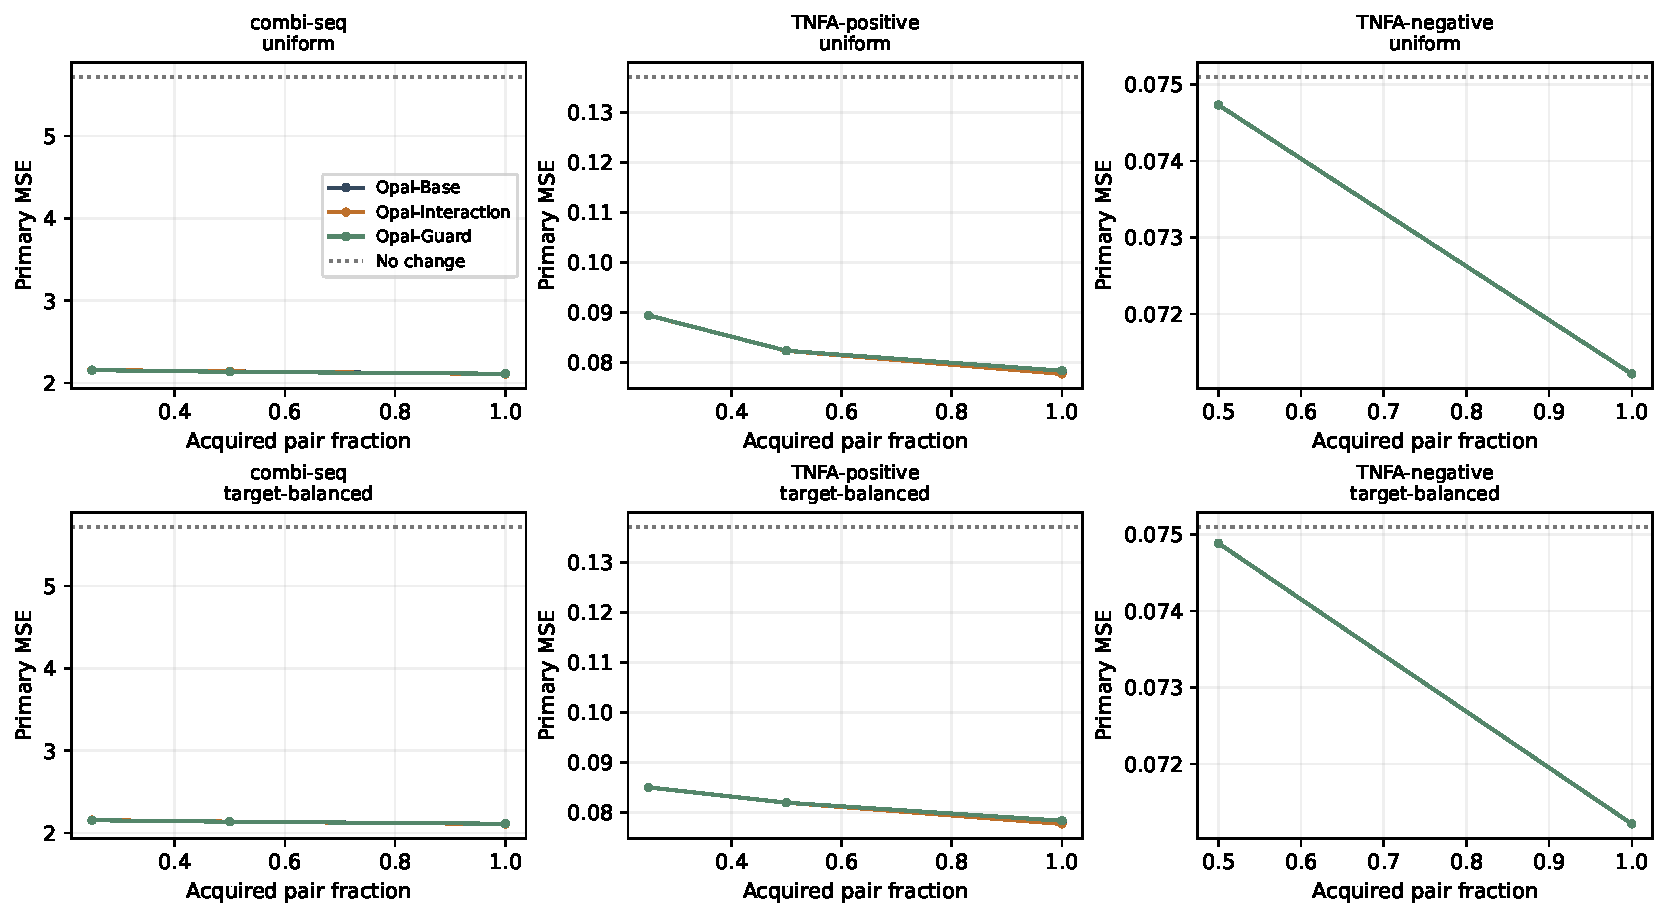
\includegraphics[width=\linewidth]{evidence/model-series-current-learning.pdf}
\caption{Frozen primary acquisition curves, averaging the three acquisition seeds within each order. Missing zero-budget supervised predictions stay unavailable. The same outer pair population is scored at every prefix; no-change is shown explicitly. Complete retrospective curves and all unavailable low-support cases are retained in compact saved records.}
\end{figure}
\begin{figure}[p]\centering
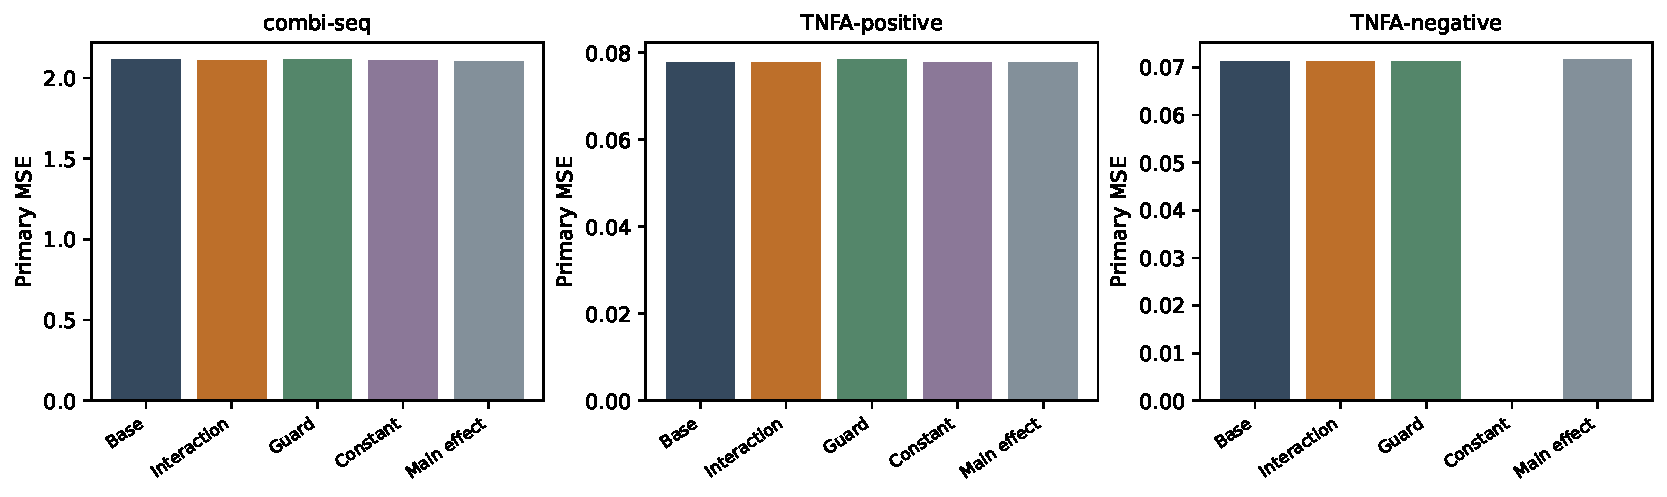
\includegraphics[width=\linewidth]{evidence/model-series-current-comparison.pdf}\par
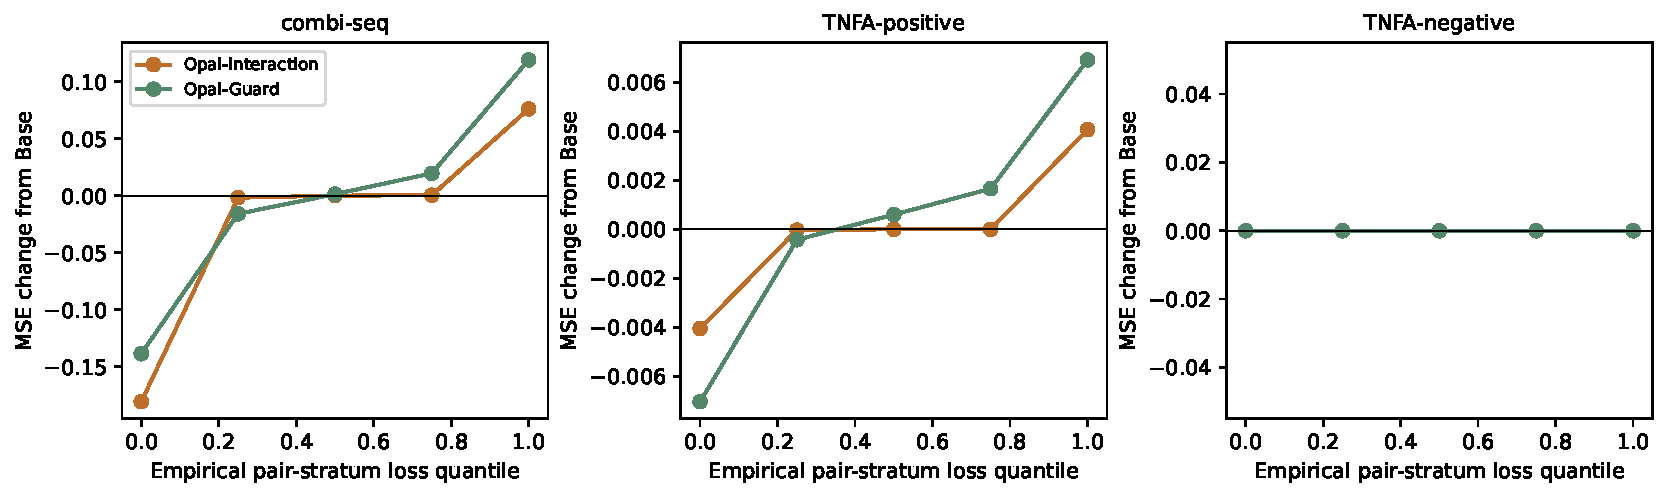
\includegraphics[width=\linewidth]{evidence/model-series-current-paired.pdf}
\caption{Primary full-label method comparison and empirical five-number summaries of paired changes from Base. The missing TNF-negative constant bar means incomplete expert availability. Pair-stratum loss distributions are not independent-pair confidence intervals.}
\end{figure}
\begin{figure}[p]\centering
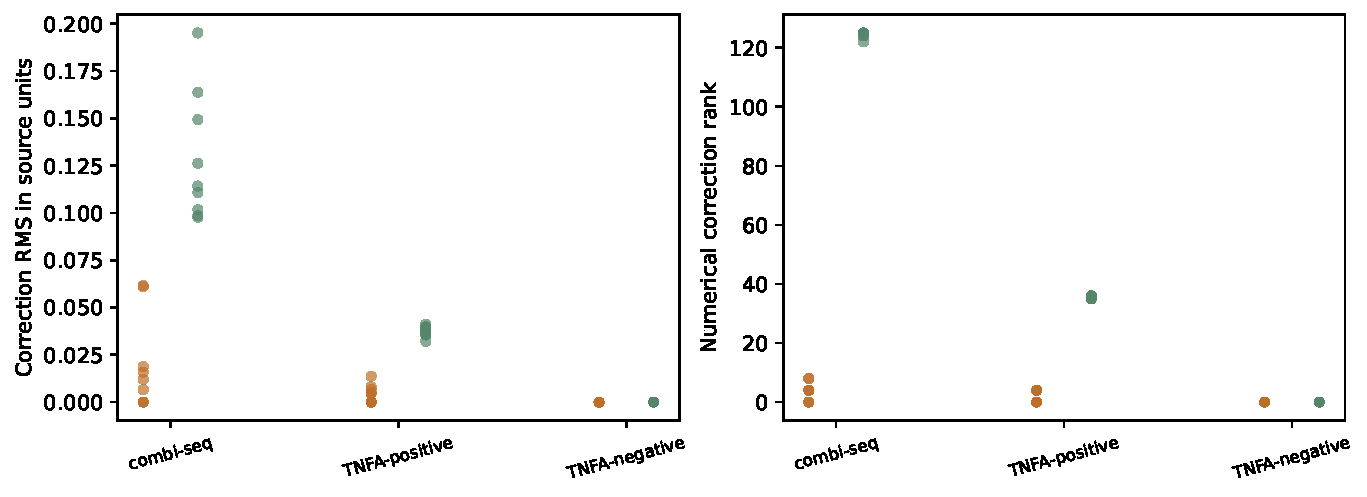
\includegraphics[width=\linewidth]{evidence/model-series-current-branches.pdf}\par
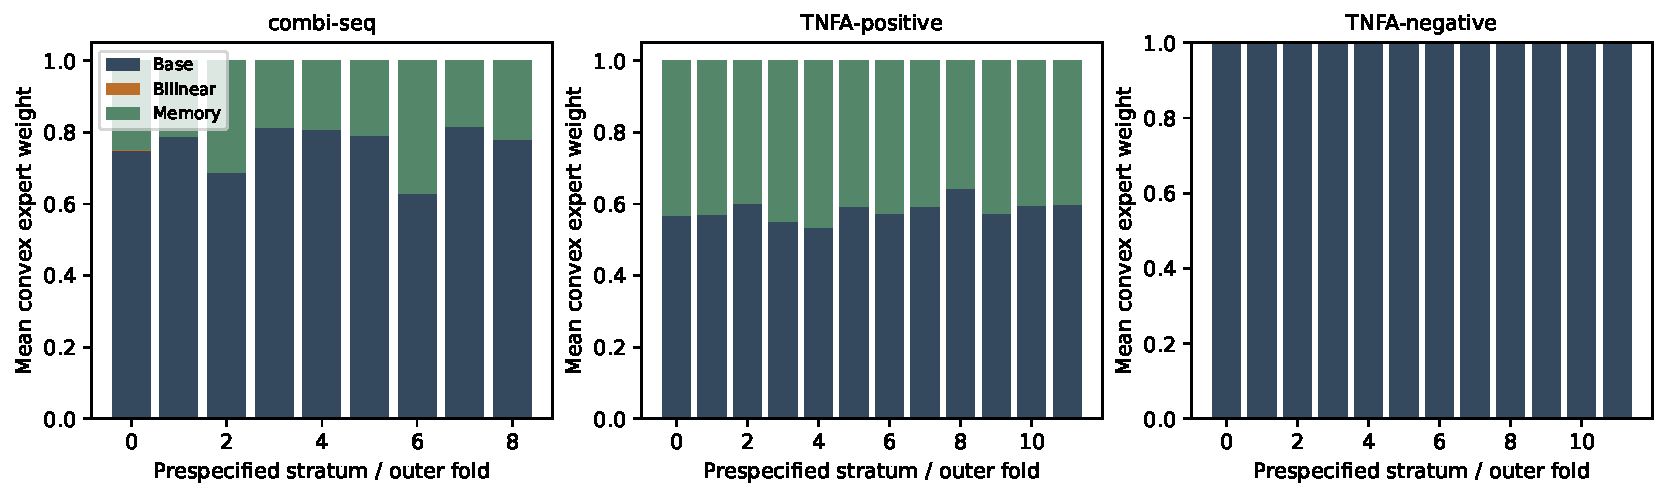
\includegraphics[width=\linewidth]{evidence/model-series-current-routing.pdf}
\caption{Saved-checkpoint correction magnitude/rank and mean convex expert weights. Zero corrections and unavailable experts remain visible. A nonzero branch or memory weight demonstrates a fitted mechanism, not biological interaction recovery.}
\end{figure}

\subsection{Executed upstream comparisons and concrete refusals}
PertSpectra's interpretable factorization uses label and graph structure \citep{chang2026}, while TxPert combines multiple knowledge graphs \citep{wenkel2026}. Strong-baseline evidence \citep{ahlmann2025} and recent calibrated-metric evidence \citep{miller2026} motivate retaining both primary MSE and discrimination diagnostics. Published correlations, outcome-selected DEG weights and technical-duplicate controls cannot populate the matched primary table or enter predictor selection.

Pinned PertSpectra, GEARS and CPA author modules execute 24 full-label TNF folds each. All 72 are protocol adaptations, not full author configurations or native frontier comparators. PertSpectra uses the unchanged factorization core, observed control/single and acquired-pair cells, without the unavailable author graph, under a two-configuration, 100-update search. Mean per-cell transformed inputs differ from Opal's transform of condition means. GEARS uses public GO plus observed-single coexpression, two hidden widths and twenty epochs. CPA uses its native Gaussian aggregate encoder/trainer, two widths, categorical presence coefficients and 120 epochs; aggregate observations are not fabricated independent cells or measured physical doses. GEARS/CPA receive all nineteen observed singles in the stratum in addition to acquired pair labels. Their control/profile input tier differs from pair-extracted observed-single fitting.

\begin{table}[htbp]\centering\small
\begin{tabular}{lrr}\toprule
Executed adaptation/reference & TNF-positive MSE & TNF-negative MSE \\\midrule
PertSpectra & 0.182326 & 0.126928 \\
GEARS & 0.093978 & 0.079552 \\
CPA & 0.113226 & 0.071731 \\
Linear, same extra observed singles & 0.082463 & 0.070020 \\
Opal-Base, primary information tier & 0.077789 & 0.071218 \\\bottomrule
\end{tabular}
\caption{Actually executed comparisons on unchanged primary endpoints. The extra-single linear control uses the same nineteen singles, one control and acquired pairs as the aggregate adaptations, with three development-selected penalties. It improves on Base in TNF-negative. Input tiers and search budgets differ, so these numbers do not rank full published configurations.}
\end{table}

Exact licensed PRESAGE GenePT and ESM vectors were already cached and reused. Native probes fail on an undefined PCA decoder, a vector-pooling call signature, and a two-row GAT output for one two-target pair. No invented aggregation or substituted random projection is scored. Public-only TxPert import fails on missing \texttt{omegaconf}; its supported Python/Torch closure is unresolved in the existing environments, and proprietary graphs are unavailable. Exact attempts and source pins are retained. Missing canonical inputs and unsupported closures prevent corresponding native competitiveness claims. State/CellFlow remain audited distributional context without copied published scores.

\subsection{Cost, usable checkpoints and limits}
The search is unequal: 24 Base references, 24 Interaction configurations plus zero, four retrieval/router settings with fully nested refits, and two native-adaptation configurations followed by selected refitting. CPU fitting uses one thread and float64; upstream adaptations use the existing Python 3.10/Torch 2.0 CUDA environment on an RTX 4060. Train/inference time, checkpoint bytes and fitted coefficient, representation, memory and support values are saved separately. Native training RAM was not captured; replay RAM is labeled reconstruction/inference RAM and cannot complete the efficiency criterion. CPU/GPU timing is not an equivalent-hardware Pareto comparison.

Safe JSON/NPZ evaluation checkpoints and content-addressed numeric-row stores retain source, scale, ordered genes, reference provenance, split, selected penalties, support and expert attribution. All evaluation checkpoints replay; the 72 upstream adaptations replay within the frozen $10^{-6}$ float32 tolerance, while Opal float64 replay uses $10^{-10}$. Historical 1,296 budget and 72 transport checkpoints also replay exactly. Later all-development refits have separate deployment manifests and no inherited evaluation score. Batch inference is allowed for deployment checkpoints; the sealed retrospective evaluator refuses them. Weights remain local because source/publication authorization for redistribution is absent. The local review package is 0.1.3.dev0; approved 0.1.2 assets are unchanged.

The owner-approved retained-artifact ceiling is 3 GB, with a 1 GiB reserve on writable C. D/E are read-only below reserve; no old files are removed. The initial 1 GB and later 2 GB pauses, retries and accounting correction remain recorded. Default promotion fails, and complete native competitiveness and efficiency criteria remain unestablished. Independent cultures, matched reference/dose provenance, biological precision/power, custody and actual laboratory validation remain external dependencies.
\begin{figure}[htbp]\centering
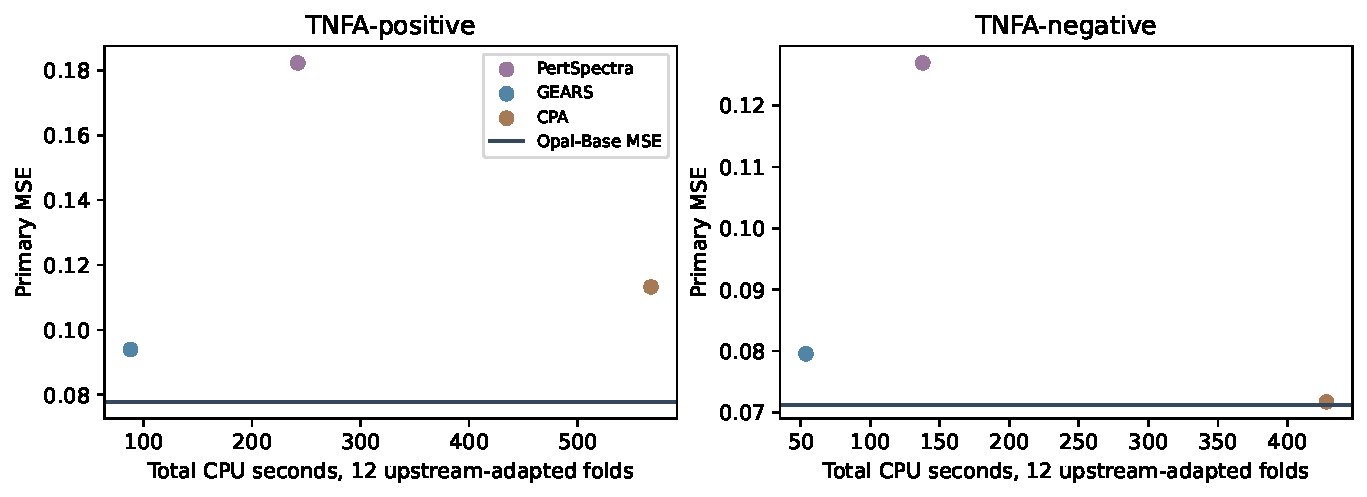
\includegraphics[width=\linewidth]{evidence/model-series-current-native-cost.pdf}
\caption{Actually executed upstream adaptations, total process CPU seconds across twelve folds in each TNF context versus primary MSE. The horizontal line is Base's MSE, not a timing comparison. GPU work and unavailable native training RAM prevent equivalent-hardware efficiency or a complete Pareto claim.}
\end{figure}
\clearpage
